\subsection{Data Extraction in PRISM}

The analytical dataset used in this study originates from the Plastic Recovery Insights Steering Model (PRISM), a data ecosystem developed by AEPW to gather country-level plastic waste, demographic, and socioeconomic data from heterogeneous public sources.

\begin{figure}[H]
	\centering
	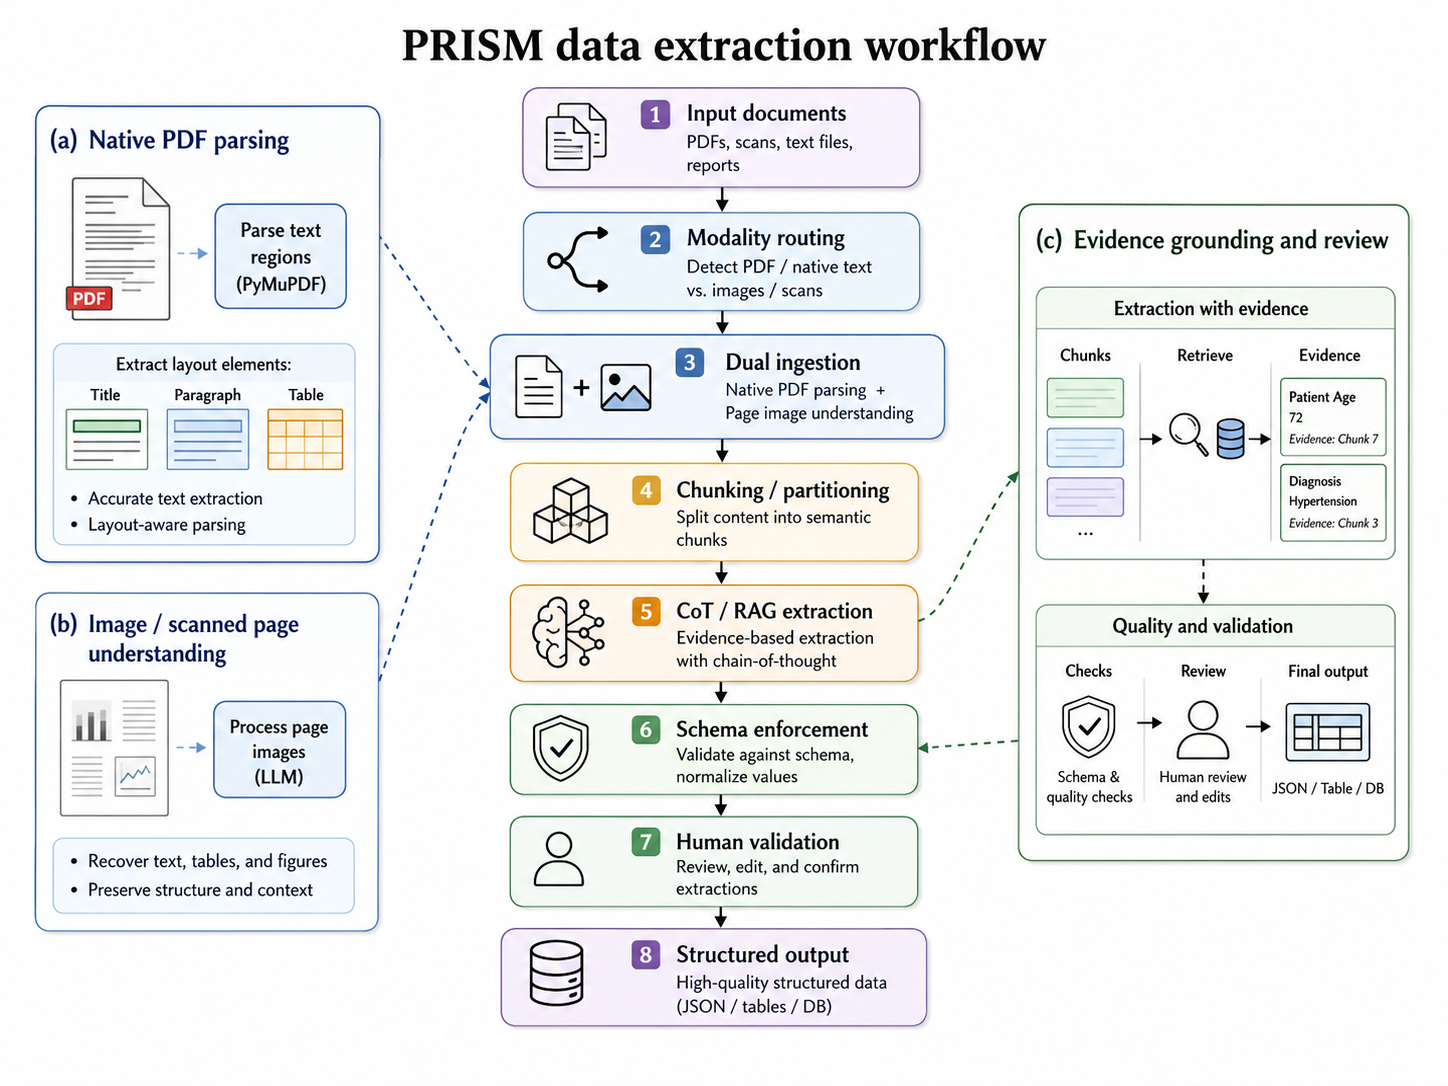
\includegraphics[width=1.0\linewidth]{figures/prism_data_extraction.png}
	\caption{
		The data extraction workflow runs through PRISM. When a document comes in, the system first identifies the document type, which is either PDF or tabular file. For PDF documents, PRISM first parses text regions using PyMuPDF and processes page images using large language models (LLMs). Then, both PDF-derived text and tabular files are partitioned into chunks. Finally, the system uses LLMs to extract data points via chain-of-thought prompting and retrieval-augmented generation. All data points undergo human validation before being used by downstream analysis.
	}
	\label{fig:prism_data_extraction}
\end{figure}

% PRISM transforms unstructured source files into structured analytical records through an LLM-assisted data extraction workflow (Figure~\ref{fig:prism_data_extraction}). Each extracted data point includes a specific location (country or region), a reference year, a numerical value, a measurement unit, a data group, and a source reference. Because automated extraction with LLMs can introduce noise and inaccuracies, all extracted records are manually reviewed and approved before being admitted into the AUDA analytical database, where they are subsequently used for modeling and visualization.

% ChatGPT
% TODO: rewrite this
Figure~\ref{fig:prism_data_extraction} illustrates the end-to-end data extraction workflow used in the PRISM platform to transform uploaded unstructured documents into validated, structured data points. The process begins when an end user uploads a document, such as a PDF or Excel file, through the platform interface. The uploaded file is stored in Azure Blob Storage, while its metadata, including file type and storage URL, is recorded in the backend database. The system then classifies the document type to determine the appropriate processing strategy. For PDF documents, textual content is parsed using PyMuPDF, while visual elements such as tables, charts, and images are interpreted using GPT-4o. For Excel documents, structured tables are divided into smaller row-wise chunks to support efficient extraction.

% ChatGPT
% TODO: rewrite this
After parsing, the PDF pipeline stores embedded text chunks in Azure AI Search to support retrieval-augmented generation for selected fields such as publisher and report date. The extraction component then applies large language models to identify relevant data points, including year, location, data point name, value, unit, and source context. The extracted outputs are subsequently passed through multiple post-processing layers, including data cleaning, location and data-point mapping, duplicate removal, unit standardization, calculated field generation, and quality score computation. Finally, the structured extraction results are saved as JSON in Azure Blob Storage and appended to the database for downstream validation, visualization, mapping, and chatbot use. Overall, the figure highlights how PRISM combines cloud storage, document parsing, vector search, generative AI, and rule-based post-processing to create a scalable and auditable data extraction pipeline.
